\documentclass{llncs}
\usepackage{graphicx}
\usepackage[caption=false]{subfig}
\usepackage[dvipsnames]{xcolor}
\usepackage{amssymb}
\usepackage{amsmath}
\newcommand{\todo}[1]{\textcolor{red}{TODO: #1}}


\title{Old or Heavy?\\Decaying Gracefully with Age/Weight Shapes.}
\titlerunning{Dynamic Strategy Priority}
\authorrunning{Reger \and Rawson}
\author{Michael Rawson \and Giles Reger}
\institute{University of Manchester, Manchester, UK}

%
%   Logical notation
%
\newcommand{\imply}{\rightarrow}
%\renewcommand{\implies}{\imply}
\newcommand{\liff}{\Leftrightarrow}
\newcommand{\lniff}{\not\Leftrightarrow}
\newcommand{\iffl}{\leftrightarrow}
\newcommand{\xor}{\otimes}
\newcommand{\orl}{\vee}
\newcommand{\bigorl}{\bigvee}
\newcommand{\andl}{\wedge}
\newcommand{\bigandl}{\bigwedge}
\newcommand{\notl}{\neg}
\renewcommand{\models}{\vDash}
\newcommand{\nmodels}{\nvDash}
\newcommand{\subst}[2]{#1 \mapsto #2}       % for substitutions
\newcommand{\Subst}[1]{\{#1\}}      % for substitutions
\newcommand{\emptysubst}{\varepsilon}
\newcommand{\true}{\mathsf{true}}      % boolean value true
\newcommand{\false}{\mathsf{false}}     % boolean value false
\newcommand{\eql}{\simeq}           % equality
\newcommand{\neql}{\not\simeq}           % equality

\begin{document}
\maketitle
\begin{abstract}
Vampire is an automatic theorem prover for first-order logic.
During proof search in given-clause algorithms, Vampire repeatedly selects clauses from either an \emph{age} or a \emph{weight} queue in a fixed, but configurable \emph{age/weight ratio} (AWR).
We show that an optimal fixed value of this ratio can produce proofs significantly more quickly on a given problem, and further that varying AWR during proof search can improve upon a fixed ratio.
Based on these observations we develop several new modes for Vampire which vary AWR according to a ``shape'' during proof search.
The modes solve a number of new problems in the TPTP benchmark.
\end{abstract}

%%%%%%%%%%%%%%%%%%%%%%%%%%%%%%%%%%%%%%%%%%%
\section{Introduction}
\label{sec:introduction}

At the core of all modern saturation-based theorem provers is \emph{clause selection}. It has been known for a long time that the way that clauses are selected in the given clause algorithm is important and early work in 80s already introduce the concept of selecting clauses as a ratio between the age and weight of a clause with the intuition that this balances between breadth and depth first search of the clause space. Whilst complex 


\cite{DBLP:conf/cade/SchulzM16}

We explore this 


After covering relevant background material in Section~\ref{sec:background} the remainder of the paper makes the following contributions:
\begin{itemize}
	\item An experimental 
	\item 
	\item An implementation of this approach in the Vampire~\cite{vampire} theorem prover and an experimental analysis demonstrating its impact. This new method for clause selection led to X
\end{itemize}
Conclusions are drawn and future work discussed in Section~\ref{sec:conclusion}.





%%%%%%%%%%%%%%%%%%%%%%%%%%%%%%%%%%%%%%%%%%%
\section{Background} \label{sec:background}

This section introduces the relevant background for the rest of the paper.

%%%%%%
\paragraph{First-Order Logic.} We consider the standard first-order predicate logic with
equality. Terms are of the form $f(t_1,\ldots,t_n), c$ or $x$ where
$f$ is a \emph{function symbol} of arity $n \geq 1$, $t_1,\ldots, t_n$ are terms, $c$ is a zero arity function symbol (i.e. a constant) and $x$ is a variable. 
%
The \emph{weight} of a term $t$ is defined as $w(t) =1$ if $t$ is a variable or a constant
and as $w(t) = 1+\sum_{i=1,\ldots,n} w(t_i)$ if $t$ is of the form
$f(t_1,\ldots,t_n)$. In other words, the weight or a term is the
number of symbols in it.
%
Atoms are of the form $p(t_1,\ldots,t_n), q$ or $t_1 \eql t_2$ where $p$ is a \emph{predicate symbol} of arity $n$, $t_1, \ldots, t_n$ are terms, $q$ is a zero arity predicate symbol and $\eql$ is the \emph{equality symbol}. 
%
The weight function naturally extends to atoms: $w(p(t_1,\ldots,t_n)) = 1+\sum_{i=1,\ldots,n} w(t_i)$, $w(t_1 \eql t_2) = w(t_1)+w(t_2)$,
and $w(q)=1$.
%
A literal is either an atom $A$, in which case we call it \emph{positive}, or a negation $\notl A$,
in which case we call it \emph{negative}.
%We write negated equalities as $t_1 \neql t_2$. 
%
The weight of a literal is the weight of the corresponding atom. 
% 
%We write $t[s]_p$ and $L[s]_p$ to denote that a term $s$ occurs in a term $t$ (in a literal $L$) at a position $p$.
%
A \emph{clause} is a disjunction of literals $L_1 \orl \ldots \orl L_n$ for $n \geq 0$.
We disregard the order of literals and treat a clause as a multiset. 
%
The weight of a clause is the sum of the weight of its literals. 

%%%%%%
\paragraph{The Given Clause Algorithm.}

Saturation-based theorem provers \emph{saturate} a set of clauses $S$ with respect to an inference system $\mathbb{I}$ e.g. they compute a set of clauses $S'$ by applying rules in $\mathbb{I}$ to clauses in $S$ until no new clauses are generated. 
%
If the empty clause is generated then $S$ is unsatisfiable.
%
Calculi such as resolution and superposition have conditions that ensure \emph{completeness}, which means that a saturated set $S$ is satisfiable if it does not contain the empty clause as an element.
%
As first-order logic is only semi-decidable, it is not necessarily the case that $S$ has a finite saturation, and even if it does it may be unachievable in practice using the available resources. 
%
Therefore, much effort in saturation-based first-order theorem proving involves 
controlling proof search to make finding the empty clause more likely (within reasonable resource bounds). 
%
One important notion is that of \emph{redundancy}, being able to remove clauses from the search space that are not required. 
%
Another important notion, the subject of this paper, are literal selections that place restrictions on the inferences that can be performed. 
%
Both notions come with additional requirements for completeness.

\todo{explain a generic given-clause algorithm; define clause age}

%%%%%%
\paragraph{Age-Weight Based Clause Selection.}

\todo{ how the ``balancing'' algorithm works internally}

%%%%%%
\paragraph{Portfolio Solvers.}

\todo{remark on portfolio modes --- more choice is (sometimes) a good thing}.

%%%%%%
\paragraph{Related Work.}

%%%%%%%%%%%%%%%%%%%%%%%%%%%%%%%%%%%%%%%%%%%
\section{Optimising Age/Weight Ratios}
\subsection{Fixed AWR}
Changing Vampire's fixed AWR has a significant effect on the number of clauses required to be processed before a proof is found.
For example, Figure \ref{fig:example-optimal-awr} shows the effect of varying AWR on an illustrative problem from TPTP: a smaller number of active clauses means that fewer clauses were processed, which in general means that a proof was found faster\footnote{
It should be noted that if a small number of clauses are extremely expensive to process it may be slower than a larger number of less-expensive clauses, but in general this is a good heuristic measure for prover performance.
It also avoids reproducibility issues involved with using system timing approaches.
}.
On this problem, a good AWR value is over 400\% better by this metric than the worst AWR value.

\begin{figure}
	\centering
	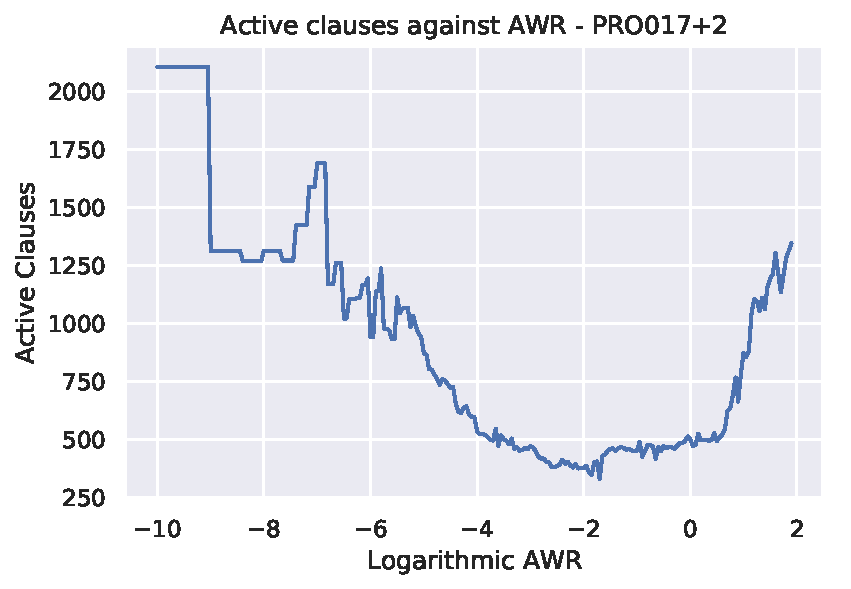
\includegraphics[width=0.8\textwidth]{example-optimal-awr}
	\caption{
The number of active clauses reported by Vampire after successful 1-second runs on a TPTP problem.
A base-2 logarithm is used to produce a continuous scale for the \(x\)-axis.
For sufficiently negative \(x\), proof search is biased towards age to such an extent that a proof is found via breadth-first search (and hence the number of active clauses remains constant), whereas after \(x\) becomes sufficiently positive, proof search does not terminate for this problem in the given time.
In between these limits, the function is ``noisy'' and discontinuous.
These properties are typical for the observed set of problems.
}
	\label{fig:example-optimal-awr}
\end{figure}

This experiment was repeated on the whole TPTP problem set, excluding problems Vampire does not support, problems which were not solved by the default mode in under a second for any AWR value, and problems solved in pre-processing.
The whole set yielded similar AWR data for 7,947 problems.
These data show that while there is no ``best'' AWR for the whole set (Figure \ref{fig:no-best-awr}), choosing a good AWR value for a problem is well-rewarded (Figure \ref{fig:optimal-awr-improvement}).

\begin{figure}
	\centering
	\begin{tabular}{l l l l l}
AWR & Minimum & Maximum & Mean & Standard Deviation\\
\hline
8:1 & 1.0 & 150.67 & 1.37 & 1.98\\
5:1 & 1.0 & 122.22 & 1.33 & 1.64\\
4:1 & 1.0 & 101.44 & 1.32 & 1.42\\
3:1 & 1.0 & 105.00 & 1.29 & 1.41\\
2:1 & 1.0 & 112.67 & 1.27 & 1.45\\
3:2 & 1.0 & 119.89 & 1.27 & 1.51\\
5:4 & 1.0 & 125.00 & 1.26 & 1.55\\
1 & 1.0 & 133.56 & 1.26 & 1.63\\
2:3 & 1.0 & 147.67 & 1.28 & 1.79\\
2 & 1.0 & 162.67 & 1.31 & 1.97\\
3 & 1.0 & 190.56 & 1.37 & 2.30\\
4 & 1.0 & 17.41 & 1.38 & 0.67\\
5 & 1.0 & 133.67 & 1.44 & 1.70\\
6 & 1.0 & 106.44 & 1.47 & 1.46\\
7 & 1.0 & 104.89 & 1.49 & 1.44\\
8 & 1.0 & 101.33 & 1.53 & 1.45\\
10 & 1.0 & 101.78 & 1.60 & 1.53\\
12 & 1.0 & 101.67 & 1.65 & 1.62\\
14 & 1.0 & 103.00 & 1.70 & 1.75\\
16 & 1.0 & 101.33 & 1.74 & 1.76\\
20 & 1.0 & 100.89 & 1.82 & 1.94\\
24 & 1.0 & 101.33 & 1.89 & 2.08\\
28 & 1.0 & 99.22 & 1.96 & 2.24\\
32 & 1.0 & 100.00 & 1.99 & 2.36\\
40 & 1.0 & 98.78 & 2.09 & 2.64\\
50 & 1.0 & 98.78 & 2.17 & 2.88\\
64 & 1.0 & 101.22 & 2.28 & 3.19\\
128 & 1.0 & 107.44 & 2.57 & 4.16\\
1024 & 1.0 & 222.01 & 2.83 & 7.55
	\end{tabular}
	\caption{The mean relative performance drop (in terms of activations compared to an optimal value) choosing a single AWR over an entire problem set causes. No setting is significantly ``better'' or ``worse'' than the others, but some have more variance in performance.}
	\label{fig:no-best-awr}
\end{figure}

\begin{figure}
	\centering
	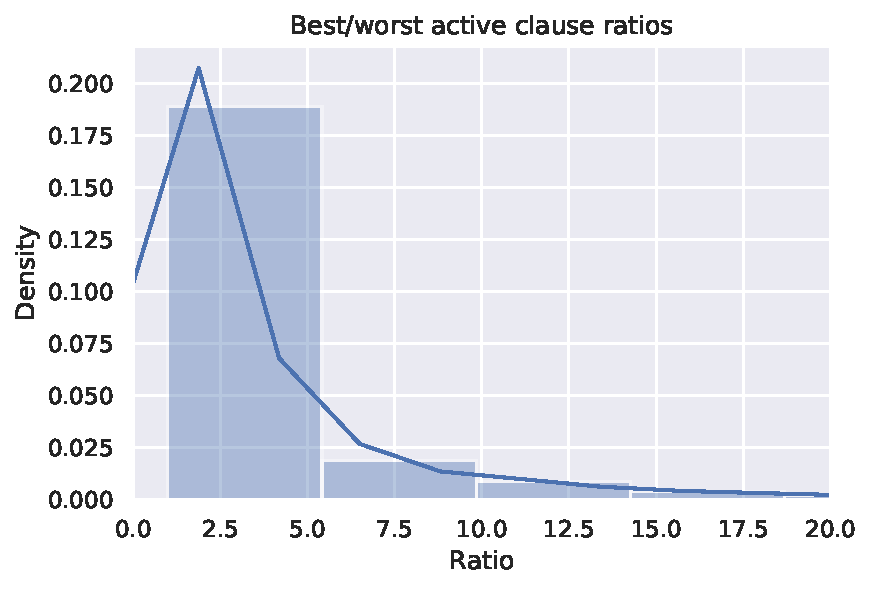
\includegraphics[width=0.8\textwidth]{optimal-awr-improvement}
	\caption{The distribution of the relative performance gain choosing the best AWR value creates, relative to the worst AWR value.}
	\label{fig:optimal-awr-improvement}
\end{figure}


\subsection{Variable AWR}
Although choosing a good AWR value is important, this is covered in part by the use of strategy scheduling~\cite{CADE18} in which many AWR values are tried in sequence (along with other prover options).
Additionally, a constant AWR fixed for the entire proof search is unlikely to be optimal for any given problem.
This can be shown by running Vampire with a randomised sequence of age/weight ratios given by a random walk repeatedly, then finding the best after a large number of repetitions.
Applying this method with 10,000 repetitions to the problem seen earlier (\texttt{PRO017+2}) yields the example AWR trend shown in Figure \ref{fig:random-walk}, which reduces the best number of activations from 330 with a fixed AWR, to 287 with a varying AWR.

In experiments, several AWR ``shapes'' were commonly seen, including:
\begin{itemize}
	\item Near-constant, as seen currently.
	\item A decreasing trend from a higher AWR to a lower AWR.
	\item An increasing trend from a lower AWR to a higher AWR.
\end{itemize}

\begin{figure}
	\centering
	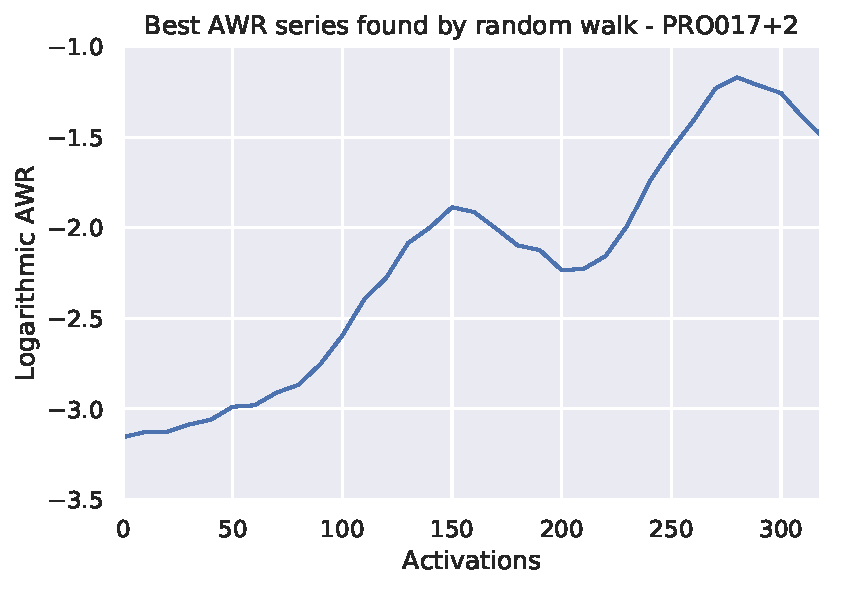
\includegraphics[width=0.8\textwidth]{random-walk}
	\caption{The AWR series that produced the lowest number of activations on a particular problem, smoothed in order to show the actual effect on proof search. This is a search strategy that a single fixed AWR cannot reproduce.}
	\label{fig:random-walk}
\end{figure}


%%%%%%%%%%%%%%%%%%%%%%%%%%%%%%%%%%%%%%%%%%%
\section{Variable AWR for Vampire}
\label{sec:variable}

If changing AWR is sometimes useful for finding proofs more quickly, this could be useful as a Vampire option.
In general we would like to describe any possible sequence that the AWR could follow during proof search.
However, some details constrain the design space:
\begin{enumerate}
	\item Changing the AWR too frequently or sharply has little effect, due to the ``balancing'' algorithm --- see Section \ref{sec:introduction}.
	\item A general (configurable) \emph{shape} is more likely to be widely applicable than a specific series of data points.
	\item The shape must extend naturally to an indefinitely-long proof search.
\end{enumerate}

In this work we selected two general trends to explore: a trend away from the original (fixed) AWR toward 1:1 (``decay''), and a trend from 1:1 toward the original setting (``converge'').
Since a simple linear shape does not extend well to indefinite proof search (it is unclear what should happen after either 1:1 or the target AWR is reached), an exponential decay function is used instead, as shown in Figure \ref{fig:decay-and-converge}.

These shapes are further parameterised by an integral \emph{shape frequency} setting, which controls the rate of decay or convergence: every \(n\) steps, the difference between the current and the target AWR is halved, rounding where necessary.
In future, this might allow the use of repeating patterns such as a sinusoid, hence \emph{frequency}.

Our approach here was restricted by the balancing algorithm used internally, as AWR steps must be discrete and do not take effect immediately.
An alternative approach might use an age/weight probability, rather than a ratio, from which age or weight decisions would be pseudo-randomly (but reproducably) taken with the use of a seeded PRNG.
This would permit use of continuous age/weight functions, but would also introduce the possibility of ``getting unlucky'' in which a clause preferred by the age/weight probability is not selected due to an improbable-but-possible series of PRNG samples.

\begin{figure}
	\subfloat{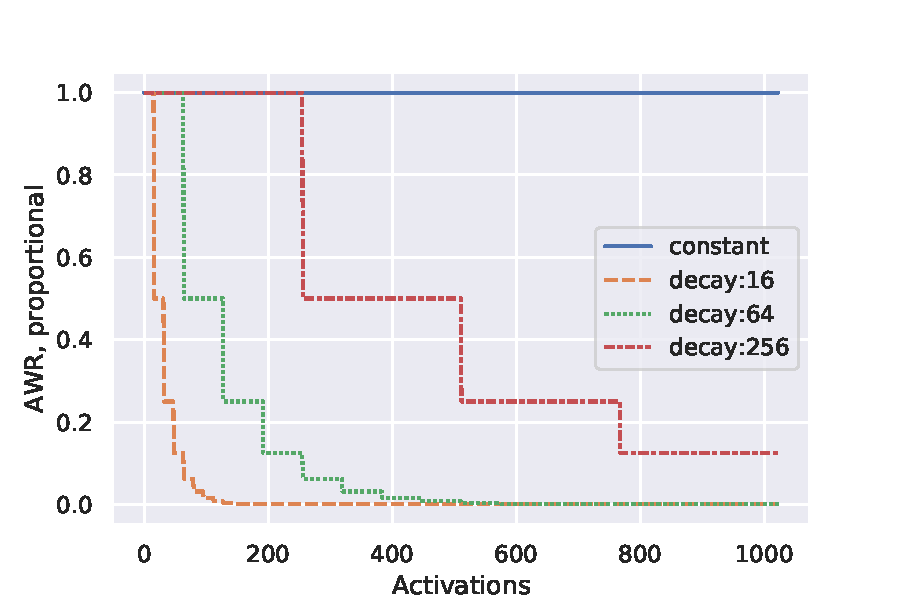
\includegraphics[width=0.5\textwidth]{shape-decay}}
	\subfloat{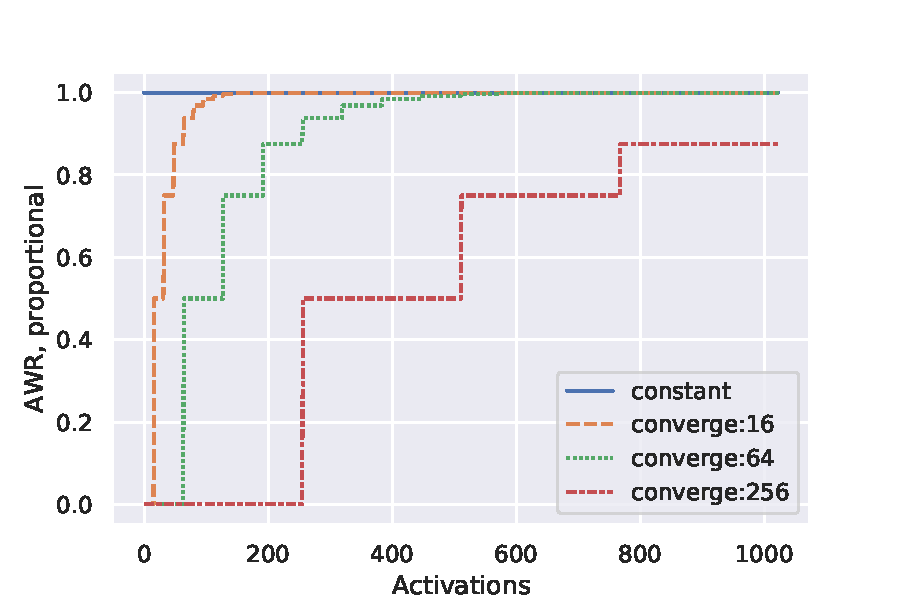
\includegraphics[width=0.5\textwidth]{shape-converge}}
	\caption{The new \emph{decay} and \emph{converge} AWR shapes as implemented in Vampire. Different curves exhibit the effect of the AWR shape frequency setting.}
	\label{fig:decay-and-converge}
\end{figure}

Together, these new settings allow a number of new option combinations, which can be used in conjunction with Vampire's portfolio \emph{CASC mode} pending integration into the strategy schedules.

\section{Experimental Evaluation}
In practice, decaying from an age-biased initial AWR to 1:1 (or converging backwards) was not found to be an improvement.
However, age/weight shapes decaying from or converging to a weight-based AWR were found to be useful in some cases.
An experimental evaluation of this approach on the TPTP~\cite{tptp} benchmark follows.

Vampire first ran to establish baseline performance in its competition \emph{CASC mode} on all problems in TPTP, with a wallclock time limit of 300 seconds.
For experimental purposes, the same environment was preserved with the exception of activating the new ``shapes'' settings with a range of different shape frequencies.
The baseline solved 13,057 problems in total.
No experimental configuration improved on this figure, but some problems not solved by baseline were solved by the new configurations, and some entirely new problems were solved.

\subsection{Raw Performance}
The following shows the performance in terms of solved problems of all the configurations tested.
These data show that configurations which are more similar to the baseline (i.e. slow decay or fast convergence) achieve more similar performance, as expected.

\begin{center}
\begin{tabular}{l l l}
	Configuration & Frequency & Proved\\
	\hline
	baseline & -- & 13057\\
	\hline
	converge & 1 & 13039\\
	converge & 5 & 13029\\
	converge & 10 & 13028\\
	converge & 50 & 13015\\
	converge & 100 & 12976\\
	converge & 500 & 12895\\
	converge & 1000 & 12837\\
	converge & 5000 & 12775\\
	converge & 10000 & 12751\\
	\hline
	decay & 1 & 12698\\
	decay & 5 & 12702\\
	decay & 10 & 12698\\
	decay & 50 & 12712\\
	decay & 100 & 12726\\
	decay & 500 & 12795\\
	decay & 1000 & 12860\\
	decay & 5000 & 12982\\
	decay & 10000 & 13002\\
\end{tabular}
\end{center}

\subsection{Uniques}
The following shows the number of problems the new configurations solved that were not solved by the baseline prover.
This shows the number of new problems that might be able to be solved if the new configurations were added to the competition mode.
In total, 134 problems were solved by the new configurations that were not solved by the baseline.

\begin{center}
\begin{tabular}{l l l}
	Configuration & Frequency & Unique\\
	\hline
	converge & 1 & 24\\
	converge & 5 & 27\\
	converge & 10 & 35\\
	converge & 50 & 45\\
	converge & 100 & 51\\
	converge & 500 & 63\\
	converge & 1000 & 52\\
	converge & 5000 & 53\\
	converge & 10000 & 53\\
	\hline
	decay & 1 & 48\\
	decay & 5 & 51\\
	decay & 10 & 48\\
	decay & 50 & 49\\
	decay & 100 & 46\\
	decay & 500 & 29\\
	decay & 1000 & 29\\
	decay & 5000 & 16\\
	decay & 10000 & 7\\
\end{tabular}
\end{center}

\subsection{New Problems}
Some problems were solved which were marked as ``Unknown'' status in the TPTP headers.
Vampire baseline (and several configurations) were able to solve \texttt{GEO120+1}, but only converging with frequency 50 solved \texttt{SET345-6} and only decaying with frequency 1 solved \texttt{LAT320+3}.


%%%%%%%%%%%%%%%%%%%%%%%%%%%%%%%%%%%%%%%%%%%
\section{Conclusions and Future Work}
\label{sec:conclusions}

\todo{this is a thing, you can do it, you should do it (?), we can probably do better}.

\todo{more shapes, better ways of doing frequency decay, integrate into existing strategy schedules}.

\bibliographystyle{plain}
\bibliography{references}
\end{document}
